\documentclass[a4paper]{article} 
\addtolength{\hoffset}{-2.25cm}
\addtolength{\textwidth}{4.5cm}
\addtolength{\voffset}{-3.25cm}
\addtolength{\textheight}{5cm}
\setlength{\parskip}{0pt}
\setlength{\parindent}{0in}

\usepackage[square,sort,comma,numbers]{natbib}
\usepackage{blindtext} % Package to generate dummy text
\usepackage{charter} % Use the Charter font
\usepackage[utf8]{inputenc} % Use UTF-8 encoding
\usepackage{microtype} % Slightly tweak font spacing for aesthetics
\usepackage{amsthm, amsmath, amssymb} % Mathematical typesetting
\usepackage{float} % Improved interface for floating objects
\usepackage{hyperref} % For hyperlinks in the PDF
\usepackage{graphicx} % Enhanced support for graphics
\usepackage{subcaption} % Required for subfigures

\usepackage{xcolor} % Driver-independent color extensions
\usepackage{pseudocode} % Environment for specifying algorithms in a natural way
\usepackage[mmddyy]{datetime} % Uses YEAR-MONTH-DAY format for dates

\usepackage{tikz}

\usepackage{fancyhdr} % Headers and footers
\pagestyle{fancy} % All pages have headers and footers
\fancyhead{}\renewcommand{\headrulewidth}{0pt} % Blank out the default header
\fancyfoot[L]{} % Custom footer text
\fancyfoot[C]{} % Custom footer text
\fancyfoot[R]{\thepage} % Custom footer text
\newcommand{\note}[1]{\marginpar{\scriptsize \textcolor{red}{#1}}} % Enables comments in red on margin

\DeclareMathOperator*{\argmin}{arg\,min}

%----------------------------------------------------------------------------------------


%-------------------------------
%	TITLE VARIABLES (identify your work!)
%-------------------------------

\newcommand{\yourname}{PICARD Emilio} % replace YOURNAME with your name
\newcommand{\youremail}{emilio.picard@free.fr} % replace YOUREMAIL with your email
\newcommand{\assignmentnumber}{1} % replace X with the lab session number

\begin{document}

%-------------------------------
%	TITLE SECTION (do not modify unless you really need to)
%-------------------------------
\fancyhead[C]{}
\hrule \medskip
\begin{minipage}{0.295\textwidth} 
\raggedright
\footnotesize
\yourname \hfill\\
\youremail
\end{minipage}
\begin{minipage}{0.4\textwidth} 
\centering 
\large 
Lab session \# \assignmentnumber\\ 
\normalsize 
ALTEGRAD 2023\\ 
\end{minipage}
\begin{minipage}{0.295\textwidth} 
\raggedleft
\today\hfill\\
\end{minipage}
\medskip\hrule 
\bigskip

%-------------------------------
%	ASSIGNMENT CONTENT (add your responses)
%-------------------------------

\section{Question 1}

\noindent
The basic self-attention mechanism is a common approach to capture semantic representations of words. This consist on creating a single attention vector. Doing though, this method cannot handle tasks like sentiment classification, as there is not much information as input.
\\
\\
\noindent
A first approach to handle this is to add a max (or average) pooling layer at all time step of the forward path. however, this could be hard to implement in a RNN structure.
\\
\\
\noindent
Another good approach to improve basic self-attention mechanism is to 
modify his input; to have more dependency in the $2D$ matrix of embeddings, before going throught the attention mechanism, it may be useful to use a bidirectional LSTM that outputs $H$, a $2D$ matix of size $n \times 2u$ (instead of having a unidirectionnal approach wich outputs a vector fo size $n$). This produces a more relevent sentence representation.
\\
\\
\noindent
Additionally, a common issue with basic self-attention is that it tends to focus on redundant information, where attention heads often concentrate on similar words or parts of the input. To mitigate this, a penalization term can be introduced to encourage diversity among attention heads and discourage redundancy. This penalization term, often implemented using the Frobenius norm, promotes the model to attend to different parts of the input, leading to better and more diverse sentence representations.


\section{Question 2}
\noindent
The paper \textit{Attention Is All You Need} introduced the Transformer model, which replaced recurrent operations (like those in RNNs and LSTMs) with self-attention mechanisms. The motivations for this change were leaded in addressing several limitations of recurrent models, particularly for tasks like machine translation and other sequence-based problems.
\\
\\
\noindent
\begin{itemize}
    \item from one time step to all time step (efficient in computing)
    \item motivation for parallel processing
    \item Long-Range Dependencies
    \item number of computational steps it takes for information from one token to influence another token. difficulty to compute gradients in backward path.
    \item more simple architecture
\end{itemize}

\section{Bonus (\textit{purpose of} \texttt{my\_patience} \textit{parameter})}
\noindent
In the context of training a neural network, the \texttt{my\_patience} variable refers to the patience parameter used in early stopping during training. Early stopping is a technique used to prevent overfitting and stop training when a model’s performance on the validation set stops improving. It can prevent also from overfitting.

\section{Question 3}
\noindent
For this question, I've decided to choose the last document of the test dataset. We can have a look at the
\texttt{sentence attention coefficients}, and also to the \texttt{words attention coefficients}.

\begin{figure}[H]
    \centering
    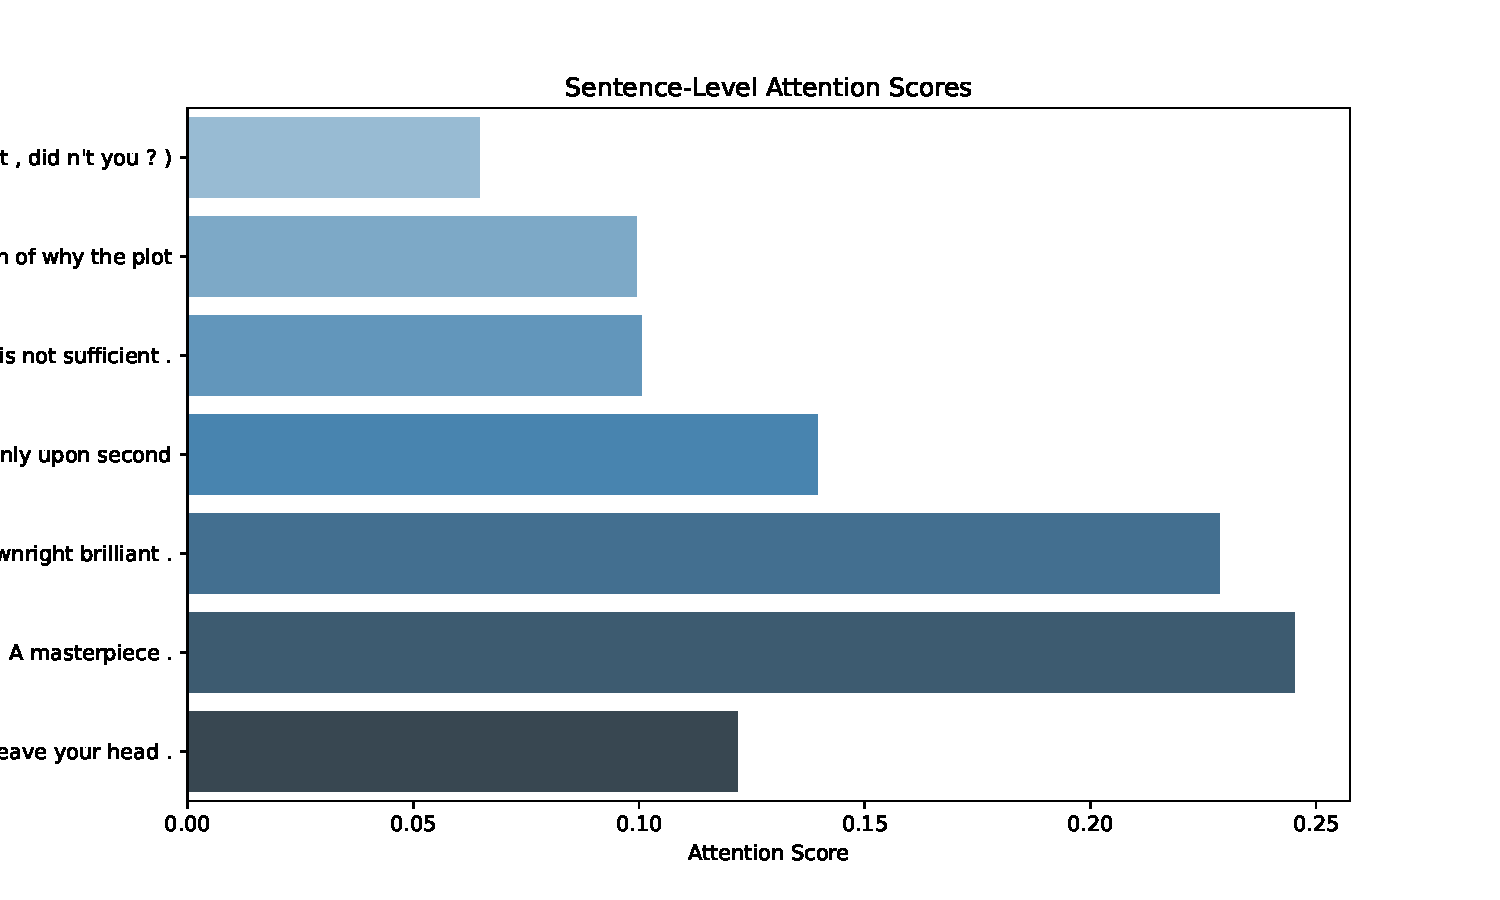
\includegraphics[width=.5\linewidth]{../figures/Sentence_attention_scores.pdf}
    \caption{Sentence attention scores for the last document of the test dataset.}
    \label{sentence-scores}    
\end{figure}

\begin{figure}[H]
    \centering
    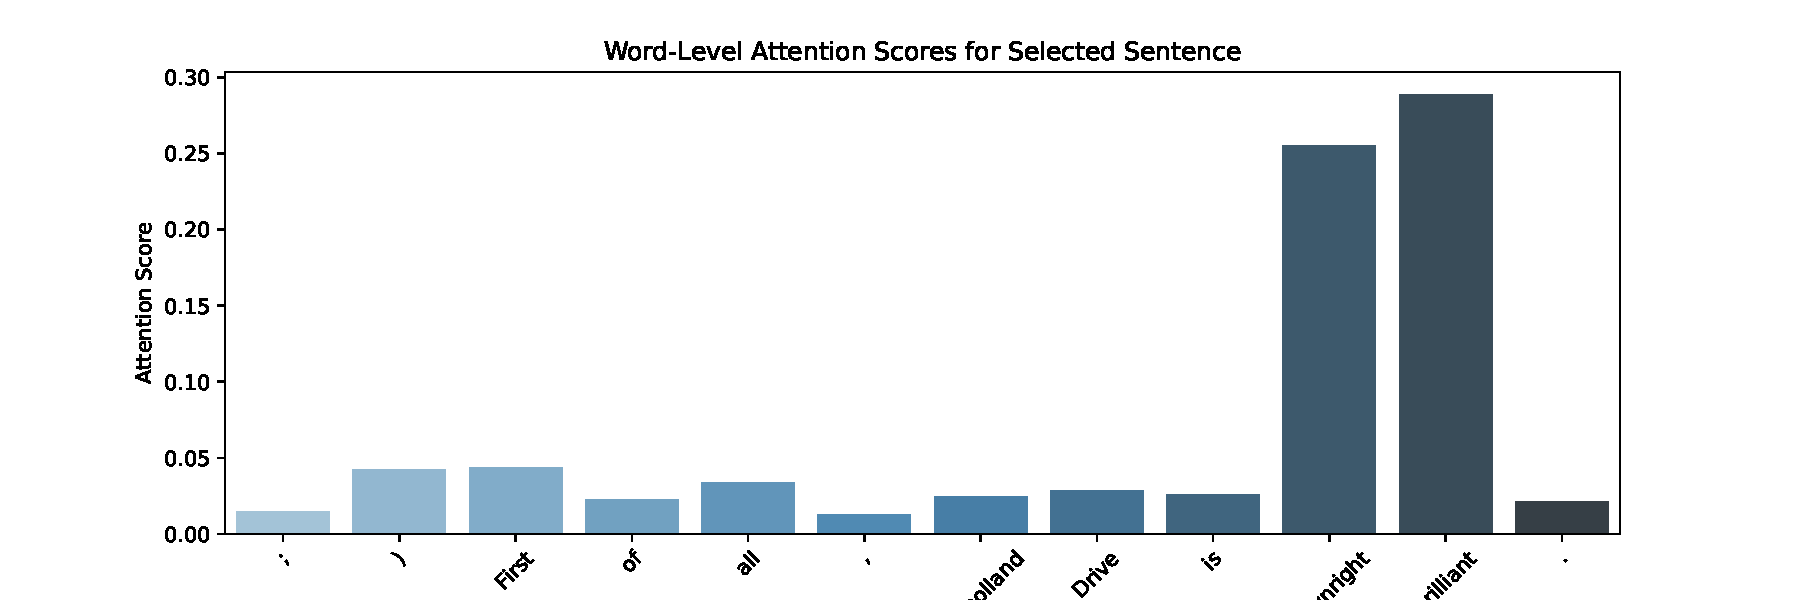
\includegraphics[width=.7\linewidth]{../figures/word_attention_scores.pdf}
    \caption{Word attention scores for the last sentence of the last document of the test dataset.}
    \label{word-scores}    
\end{figure}


\noindent
In figure \ref{sentence-scores}, we can interpret that the $5^{th}$ and $6^{th}$ sentences are the most determinents
in the choice of the model, helping it to classify if it's a good or bad review. In this case, the words
\textit{brillant} and \textit{masterpiece} might be gamechanger in the classification.  
\\
\\
\cite{vaswani2017attention}

%------------------------------------------------

\bibliographystyle{plain}
\bibliography{references} % citation records are in the references.bib document

\end{document}
